% PREAMBLE
%% 1. 文書クラス
\documentclass[11pt,a4j,onecolumn]{jsreport} % 日本語の論文を,本文フォント 11pt,A4用紙,一段組みのオプション付きで

%% 2. パッケージのインポート
\usepackage[dvipdfmx]{graphicx} % 図の挿入
\usepackage[dvipdfmx]{color}% 色の使用
\usepackage{amsmath,amssymb,amsfonts,mathrsfs} % 数式全般
\usepackage{bm}             % ベクトルなどの太字
\usepackage{cite}           % 文献番号の整理
\usepackage{siunitx}        % 単位表記
\usepackage{url}            % URLの表示
\usepackage{algorithmic}    % アルゴリズム(擬似コード)
\usepackage{listings,jvlisting} % ソースコード
\usepackage{geometry}       % ページのデザイン
\usepackage{titlesec}       % 見出しデザイン
\usepackage{fancyhdr}       % ヘッダ・フッタデザイン
\usepackage[ipaex]{pxchfon} % 日本語フォント設定
\usepackage[dvipdfmx]{hyperref}% ハイパーリンクの作成
\usepackage{pxjahyper} % (u)pLaTeXのときのみかく

%% 3. デザイン
\geometry{top=30truemm,bottom=30truemm,left=25truemm,right=25truemm} % ページ余白設定
\setlength{\headheight}{16pt}  % ヘッダー領域の高さを16ptに設定

\makeatletter  % 「@」を含む内部コマンド(\@cite など)を再定義できるようにする
  \renewcommand{\@cite}[1]{\textsuperscript{#1)}} % 引用番号を上付きで「1)」のように表示
\makeatother  % \makeatletter の終了

\titleformat{\chapter}{\normalfont\LARGE\bfseries}{\S \ \thechapter }{1em}{} % 章タイトルの書式設定:「§ 1 タイトル」のように表示
\renewcommand{\chaptermark}[1]{\markboth{\S\ \normalfont\thechapter\ ~~#1}{}} % 章見出し(ヘッダー表示用)の再定義

\newcommand{\sectionbreak}{\clearpage} % sectionごとに改ページ

\renewcommand{\figurename}{\sffamily Fig.~} % 図タイトルのフォント
\renewcommand{\tablename}{\sffamily Table~} % 表タイトルのフォント


\hypersetup{ % ハイパーリンクのセットアップ
 setpagesize=false,
 bookmarks=true,
 bookmarksdepth=tocdepth,
 bookmarksnumbered=true,
 hidelinks}

\lstset{
  basicstyle=\scriptsize\ttfamily, % ソースコードのデザイン
  numbers=left,
  frame=single
  keywordstyle=\color{blue}\bfseries,
  commentstyle=\color{gray},
  stringstyle=\color{green},
}

%% 4. 独自記号の定義(頻出する記号の書き方をここで定義することで手間を短縮)

\newcommand*{\Romannumeral}[1]{\uppercase\expandafter{\romannumeral#1}}

\newcommand*{\Si}[2]{$#1\ [\si{#2}]$}



%=====================================================================================
%=====================================================================================

% DOCUMENT
\begin{document}


%=====================================================================================

%% 5. タイトルページの作成
\begin{titlepage}
\centering

\vspace{20truemm}
{\Large\noindent 東京大学工学部建築学科 卒業論文}\\
\vspace{40truemm}
{\huge\noindent\textbf{\LaTeX を導入して}}\\
\medskip
{\huge\noindent\textbf{卒業論文を書いてみよう!}}\\
\vspace{\baselineskip}
{\large\noindent\textbf{(Let's Write a Graduation Thesis}}\\
\medskip
{\large\noindent\textbf{Using \LaTeX !)}}\\
\vspace{48truemm}

{\Large\noindent
  2025年11月??日提出\\
  \vspace{8truemm}
  指導教員 糸井~達哉~准教授,小山~毅~特任准教授}\\
\vspace{16truemm}
{\large\noindent
  東京大学工学部建築学科 \\
  \vspace{4truemm}
  学籍番号 03-FFFFFF\\
  \vspace{6truemm}
  信頼性~太郎\\
  \vspace{2truemm}
  Taro SHINRAISE \\
}

\end{titlepage}

\thispagestyle{empty}
\clearpage

%=====================================================================================

%% 6. 目次の作成
\pagenumbering{roman} % ページ番号を小文字ローマ数字に
\tableofcontents      % 目次出力

%=====================================================================================

%% 7. 本文の作成
\newpage
\pagestyle{fancy}
\pagenumbering{arabic}% ページ番号をアラビア数字に
\setcounter{page}{1}  % ページ数カウンターをリセット



\chapter{序論}

\subsubsection{この資料の使い方}

本ファイルは\LaTeX のチュートリアル兼卒論テンプレートです.
文書の枠組みや図表等を作成する際に型として使用していただけたら幸いです.
また,実際に手を動かしてこの.texファイルを編集し,\TeX 打ちの練習を行ってみてください.

より高度な使い方はChatGPTやサイトを検索して調べてください.


\section{卒論本文作成要項}

卒論本文の体裁は表紙に書かなければならない内容くらいしか決まっていないので,テンプレートを自由にいじってデザインしましょう.
ただし,ヘッダーやフッタの体裁の一般的な慣習や,ページ数の振り方の決まり(目次・本文・付録でカウンターをリセットすること)は守りましょう.
デザインのコツとして,
1. 図表はページの半分くらいを使って大きく表示すること,
2. 節(section)ごとにページを改めること(すでにプリアンブルで設定しています),
3. 文字の大きさ・行間にゆとりを設けること,
4. 図表の文字サイズは本文とそろえること~
が挙げられます.

\section{TeX作業の基本}

\subsection{環境構築}

研究室GitHubの「
\href{https://github.com/ItoiLab/Itoilab-setup-guide/blob/main/Itoilab-setup-guide.md#latex%E3%81%AE%E5%B0%8E%E5%85%A5}{セットアップリポジトリ}
\cite{itoilab2025}」を参照のこと.\\
\hspace{10em}↑ハイパーリンクになっています.クリックしてリンク先に飛んでください

VSCode内での作業がおすすめです.画面左に.texファイル,画面右に.pdfファイルを配置しましょう.
緑色の再生ボタンをクリックするとtexファイルのコンパイル,保存,pdfの更新等を自動でやってくれます.\\

あと,「
\href{https://www.jabref.org/}{JabRef}
」なるソフトをインストールしておくと参考文献の管理に便利です.

\subsection{TeX作業の流れ}

TeX作業は,
\begin{center}
  文章等の記述 → コンパイル → 出力の確認
\end{center}
のローテーションをこまめに回すことがコツとなります.
プリアンブル(節~\ref{sec:texfile}~を参照)を少しいじったり,少し何かを削ったり,順番を入れ替えたりするだけでコンパイルが通らなくなり,
pdfに出力できなくなる危険性があります.
取り返しのつく範囲内の編集を少しずつ行うことを心掛けましょう.

% 「%」の後ろに続けて書かれた文字はコメントアウトされます.
% よって,この文はpdfファイルの方では書かれていません.

また,目次・参照・図表番号等,内容によっては二回以上のコンパイル作業をしないと反映されない機能もあるので注意が必要です.\\

山本氏のサイト\cite{yamamotoHP}で\TeX に関して非常によくまとめられているので,論文執筆の際は手元に用意しておくとよいと思います.

\section{.texファイルの構成}
\label{sec:texfile}

.texファイルは「プリアンブル」と本文によって構成されます.

プリアンブルでは文書に関するさまざまな設定を行い,ここで 1. 文書の分類,2. パッケージのインポート,3. デザイン設定,
4. 独自記号の定義~等を行います.詳細は本.texファイルを眺めてください.

本文は~\textbackslash begin\{document\}~と~\textbackslash end\{document\}~の間に記述します.
ちなみに,この~\textbackslash begin\{A\}~と~\textbackslash end\{A\}~に囲まれた部分を「A環境」と呼びます.
表紙,目次,本文,参考文献,付録等により構成され,それぞれいろいろな呪文を唱える必要がありますが,
基本的には本.texファイルを参考にすればよいかと思われます.

%=====================================================================================

\chapter{文章を書く}

\section{章・段落}
ここでは,章や段落の作り方を解説します.

\subsection{章立て}

文書クラスによって異なりますが,章(\textbackslash chapter\{章名\}),節(\textbackslash section\{節名\}),小節(\textbackslash subsection\{小節名\}),
小々節(\textbackslash subsubsection\{小々節名\})~を作ることができます.
\subsubsection{番号はついていませんが,}
これが小々節です.

\subsection{段落}

.texファイルを見たらわかるように,
.texファイル上で単に改行してもpdf上では改行は反映されません.
バックスラッシュ2個\\ (\textbackslash\textbackslash) \\
で強制的に改行を行うことができます.この際段落は変わりません.(よってインデントも変わりません)

段落を変えるには,.texファイル上で空行を設けてください.\\

バックスラッシュ2個を段落終わりに配置して,pdfファイル上で空行を設けることも簡単にできます.

\section{文字}

\subsection{書体}

本文中でこのようにして~\textbackslash textbf\{\textbf{太字} \}~にすることもできます.
あまりその必要が生じる場面はないと思いますが.
数学・物理の変数を書きたいときは後に説明する別の方法をとりましょう.\\

表紙に使っている方法で,{\Huge でかい文字を書いたり}{\tiny ちっこい文字を書いたり}もできますが,
用途は限定的だと思います.

\subsection{特殊文字}

空~~~~~~~~~~~~~~~白は~「\textasciitilde」~により~明示的に表記~できます.\\

バックスラッシュ「\textbackslash」やアンパサンド「\&」,パーセント「\%」など,そのまま書くとエラーになってしまう文字がいくつかあります.
エスケープするなどの方法で書くことができます.以下にその例を示します.

\begin{tabbing}
  \hspace{20truemm} \= \hspace{10truemm} \= \hspace{30truemm} \= \hspace{10truemm} \= \hspace{30truemm} \= \hspace{10truemm} \= \hspace{20truemm} \kill
  \> 出力 \> 入力 \> 出力 \> 入力 \> 出力 \> 入力 \\
  \> \% \> \textbackslash\% \> \& \> \textbackslash\& \> \$ \> \textbackslash\$ \\
  \> \# \> \textbackslash\# \> \{ \> \textbackslash\{ \> \} \> \textbackslash\} \\
  \> \_ \> \textbackslash\_ \> \textbackslash \> \textbackslash textbackslash \> \textbar \> \textbackslash textbar \\
  \> \textendash \> \textbackslash textendash \> \textgreater \> \textbackslash textgreater \> \textless \> \textbackslash textless \\
  \> \textasciitilde \> \textbackslash textasciitilde \> \textasciiacute \> \textbackslash textasciiacute \> \textasciibreve \> \textbackslash textasciibreve \\
\end{tabbing}

\section{箇条書き}

\subsection{通常の箇条書き}

\textbackslash begin\{itemize\}~と~\textbackslash end\{itemize\} に挟まれた空間に箇条書きの要素を記述します.
各要素は \textbackslash item の後に続けて記述します.\\

入力
\begin{verbatim}
  \begin{itemize}
    \item 2016年熊本地震
    \item 2024年能登半島地震
  \end{itemize}
\end{verbatim}

出力

\begin{itemize}
  \item 2016年熊本地震
  \item 2024年能登半島地震
\end{itemize}

\textbackslash item[記号] と書いて任意の記号を用いた箇条書きができます.
また,箇条書きを入れ子にすることもできます.

\begin{itemize}
  \item[◇] 自然災害
  \begin{itemize}
    \item[○] 気象災害
    \begin{itemize}
      \item 内水氾濫
      \item 高潮
    \end{itemize}
    \item[○] 地震
    \item[○] 火山噴火
  \end{itemize}
  \item[◇] 人為災害
\end{itemize}

\subsection{番号付きの箇条書き}

\textbackslash begin\{enumerate\}~と~\textbackslash end\{enumerate\} に挟まれた空間に箇条書きの要素を記述します.
各要素は \textbackslash item の後に続けて記述します.

\begin{enumerate}
  \item 2016年熊本地震
  \item 2024年能登半島地震
\end{enumerate}


\section{物理量,数値,単位など}

\subsection{物理量}

数式や物理記号は「数式環境」内で書かなければなりません.
本節では,文章中に出てくる短い式などを書く方法を説明しています.

本文中に数式環境を作るには~\$ 1234 \$~のようにドルマークで囲うのが簡単です.
数式環境内でアルファベットを入力するとイタリックで出力され,物理量等の変数を書くのに適したフォントになります.
なお,数式の詳しい記法等は\ref{sec:math}章で説明しています.\\
\hspace{3em} 例)$f(x)$,$P(a|b)$,$2g$

\subsection{数値}

\textbackslash num\{数字\} と記述して見やすく数字を表記することができます.
浮動小数点表示や有効数字なども直感的な記述で扱うことができます.\\
\hspace{3em} 例)\num{101300.35672},\num{1.3d-2},\num{5.7e4},\num{2.26 +- 0.01},\num{12.4}\%

\subsection{単位}

単位はイタリックにしてはならず,物理量と単位の間にスペースを設けるのが決まりです.
単位を簡単に記述できるパッケージを既にインポートしているのでそんなことは考えずに記述してしまいましょう.

\subsubsection{単位単体の場合}

\textbackslash si\{単位\} と記述して単位単体を書くことができます.\\
\hspace{3em} 例)\si{mm},\si{kg~m~s^{-2}},\si{Gal}

\subsubsection{数値とセットの場合}

\textbackslash SI\{数値\}\{単位\} と記述して数字と一緒に書くことができます.\\
\hspace{3em} 例)\SI{10000}{mm},\SI{2.0E-2}{kg~m~s^{-2}},\SI{600}{Gal}

\subsubsection{物理量とセットの場合}

\textbackslash Si\{物理量\}\{単位\} と記述して物理量と一緒に書くことができるようにマクロで定義しました.\\
\hspace{3em} 例)\Si{L}{mm},\Si{F}{kg~m~s^{-2}},\Si{X_0}{Gal}

%=====================================================================================

\chapter{数式を書く}
\label{sec:math}

\section{数式環境}

数式を記述するには,ドルマークで囲った数式環境を本文中に入れるか,下記で説明する方法で数式専用の空間を確保します.

専用の空間を作る数式環境にはいくつか選択肢があるみたいですが,align 環境でだいたいうまくいくと思います.
\textbackslash begin\{align\}~と~\textbackslash end\{align\} の間に数式を記述します.
\textbackslash label\{ラベル\} により数式に名前を付けておくことをおすすめします.\\

入力
\begin{verbatim}
  \begin{align}
    \label{a_plus_b}
    a + b = 0
  \end{align}
\end{verbatim}

出力
\begin{align}
  \label{a_plus_b}
  a + b = 0
\end{align}

式変形等のために複数行にわたって書きたい場合は \& 記号で縦位置を揃えることができます.
最終行以外には \textbackslash\textbackslash を付けて改行とします.
\textbackslash notag により式番号を省略することができます.\\

入力
\begin{verbatim}
  \begin{align}
    \label{b_eq_-a}
    a + b &= 0 \notag \\
    b &= -a
  \end{align}
\end{verbatim}

出力
\begin{align}
  \label{b_eq_-a}
  a + b &= 0 \notag \\
  b &= -a
\end{align}

\section{記法}

\subsection{文字}

\subsubsection{下付き文字・上付き文字}

装飾される文字の後ろに,下付き文字なら「\_」,上付き文字なら「\^{}」と続けます.
装飾する文字が複数の場合はそれらを\{\}で囲う必要があります.

\begin{tabbing}
  \hspace{20truemm} \= \hspace{10truemm} \= \hspace{30truemm} \= \hspace{10truemm} \= \hspace{30truemm} \= \hspace{10truemm} \= \hspace{20truemm} \kill
  \> 出力 \> 入力 \> 出力 \> 入力 \> 出力 \> 入力 \\
  \> $x^2$ \> x\^{}2 \> $a_{ij}$ \> a\_\{ij\} \> $n_{12}^*$ \> n\_\{12\}\^{}* \\
\end{tabbing}

\subsubsection{アクセント}

さまざまなアクセント記号を文字に装飾するためのコマンドが用意されています.ここでは代表的なものを紹介します.

\begin{tabbing}
  \hspace{20truemm} \= \hspace{10truemm} \= \hspace{30truemm} \= \hspace{10truemm} \= \hspace{30truemm} \= \hspace{10truemm} \= \hspace{20truemm} \kill
  \> 出力 \> 入力 \> 出力 \> 入力 \> 出力 \> 入力 \\
  \> $\hat{x}$ \> \textbackslash hat\{x\} \> $\dot{x}$ \> \textbackslash dot\{x\} \> $\vec{x}$ \> \textbackslash vec\{x\} \\
  \> $\tilde{x}$ \> \textbackslash tilde\{x\} \> $\acute{x}$ \> \textbackslash acute\{x\} \> $\bar{x}$ \> \textbackslash bar\{x\} \\
\end{tabbing}

\subsubsection{ギリシャ文字}

\textbackslash の後に小文字なら小文字から,大文字なら大文字から始めるアルファベット名を記述します.
頭にvarを付けると,一部のアルファベットは別の字形になります.
偏微分で使う $\partial$ は,\textbackslash partial と入力できます.

\begin{tabbing}
  \hspace{20truemm} \= \hspace{10truemm} \= \hspace{30truemm} \= \hspace{10truemm} \= \hspace{30truemm} \= \hspace{10truemm} \= \hspace{20truemm} \kill
  \> 出力 \> 入力 \> 出力 \> 入力 \> 出力 \> 入力 \\
  \> $\Lambda$ \> \textbackslash Lambda \> $\phi$ \>\textbackslash phi \> $\varphi$ \> \textbackslash varphi \\
  \> $\epsilon$ \> \textbackslash epsilon \> $\varepsilon$ \>\textbackslash varepsilon \> $\partial$ \> \textbackslash partial \\
\end{tabbing}

\subsubsection{字体}

デフォルトのイタリックの字体以外を必要に応じて使用できます.
なお,対数logや極限limなどにはのちに説明する専用の記号が用意されているので,ここに示すローマン体に直す記法を使わないでください.

\begin{tabbing}
  \hspace{20truemm} \= \hspace{10truemm} \= \hspace{30truemm} \= \hspace{10truemm} \= \hspace{30truemm} \= \hspace{10truemm} \= \hspace{20truemm} \kill
  \> 出力 \> 入力 \> 出力 \> 入力 \> 出力 \> 入力 \\
  \> $\mathrm{a}$ \> \textbackslash mathrm\{a\} \> ${\bm a}$ \> \{\textbackslash bm a \} \> $\mathbf{a}$ \> \textbackslash mathbf\{a\} \\
  \> $\mathbb{A}$ \> \textbackslash mathbb\{A\} \> $\mathcal{A}$ \> \textbackslash mathcal\{A\} \> $\mathscr{A}$ \> \textbackslash mathscr\{A\} \\
\end{tabbing}

\subsection{演算子・関数など}

記法の例を下記列挙します.
$\log$ や $\sum$ など記号の上下に情報を付加するときは,\_ や \^{~} を付け足して柔軟に記述できます.
なお,この場合のデザインは align 環境内と本文中に書き込む場合とで異なります.

\subsubsection{算術}

\begin{tabbing}
  \hspace{20truemm} \= \hspace{10truemm} \= \hspace{30truemm} \= \hspace{10truemm} \= \hspace{30truemm} \= \hspace{10truemm} \= \hspace{20truemm} \kill
  \> 出力 \> 入力 \> 出力 \> 入力 \> 出力 \> 入力 \\
  \> $+$ \> + \> $-$ \> - \> $\pm$ \> \textbackslash pm \\
  \> $*$ \> * \> $\cdot$ \> \textbackslash cdot \> $\times$ \> \textbackslash times \\
  \> $\div$ \> \textbackslash div \> $\odot$ \> \textbackslash odot \> $\nabla$ \> \textbackslash nabla \\
\end{tabbing}

\subsubsection{集合}

\begin{tabbing}
  \hspace{20truemm} \= \hspace{10truemm} \= \hspace{30truemm} \= \hspace{10truemm} \= \hspace{30truemm} \= \hspace{10truemm} \= \hspace{20truemm} \kill
  \> 出力 \> 入力 \> 出力 \> 入力 \> 出力 \> 入力 \\
  \> $\cap$ \> \textbackslash cap \> $\cup$ \> \textbackslash cup \> $\setminus$ \> \textbackslash setminus \\
\end{tabbing}

\subsubsection{関係}

\begin{tabbing}
  \hspace{20truemm} \= \hspace{10truemm} \= \hspace{30truemm} \= \hspace{10truemm} \= \hspace{30truemm} \= \hspace{10truemm} \= \hspace{20truemm} \kill
  \> 出力 \> 入力 \> 出力 \> 入力 \> 出力 \> 入力 \\
  \> $=$ \> = \> $\neq$ \> \textbackslash neq \> $\propto$ \> \textbackslash propto \\
  \> $\simeq$ \> \textbackslash simeq \> $\sim$ \> \textbackslash sim \> $\approx$ \> \textbackslash approx \\
  \> $>$ \> \textgreater \> $\geq$ \> \textbackslash geq \> $\supset$ \> \textbackslash supset \\
  \> $<$ \> \textless \> $\leq$ \> \textbackslash leq \> $\subset$ \> \textbackslash subset \\
  \> $\in$ \> \textbackslash in \> $\parallel$ \> \textbackslash parallel \> $\perp$ \> \textbackslash perp \\
  \> $\rightarrow$ \> \textbackslash rightarrow \> $\Rightarrow$ \> \textbackslash Rightarrow \> $\Leftrightarrow$ \> \textbackslash Leftrightarrow \\
\end{tabbing}

\subsubsection{雑多}

\begin{tabbing}
  \hspace{20truemm} \= \hspace{10truemm} \= \hspace{30truemm} \= \hspace{10truemm} \= \hspace{30truemm} \= \hspace{10truemm} \= \hspace{20truemm} \kill
  \> 出力 \> 入力 \> 出力 \> 入力 \> 出力 \> 入力 \\
  \> $\infty$ \> \textbackslash infty \> $\exists$ \> \textbackslash exists \> $\forall$ \> \textbackslash forall \\
  \> $\dots$ \> \textbackslash dots \> $\because$ \> \textbackslash because \> $\therefore$ \> \textbackslash therefore \\
  \> $\top$ \> \textbackslash top \> $\varnothing$ \> \textbackslash varnothing \> $\mathbf{0}$ \> \textbackslash mathbf\{0\} \\
\end{tabbing}

\subsubsection{分数・累乗根}

\begin{tabbing}
  \hspace{20truemm} \= \hspace{10truemm} \= \hspace{30truemm} \= \hspace{10truemm} \= \hspace{30truemm} \= \hspace{10truemm} \= \hspace{20truemm} \kill
  \> 出力 \> 入力 \> 出力 \> 入力 \> 出力 \> 入力 \\
  \> $\frac{a}{b}$ \> \textbackslash frac\{a\}\{b\} \> $\sqrt{a}$ \> \textbackslash sqrt\{a\} \> $\sqrt[b]{a}$ \> \textbackslash sqrt[b]\{a\} \\
\end{tabbing}

\subsubsection{ローマン体のアルファベットを用いる演算子}

\begin{tabbing}
  \hspace{5truemm} \= \hspace{20truemm} \= \hspace{25truemm} \= \hspace{20truemm} \= \hspace{25truemm} \= \hspace{20truemm} \= \hspace{25truemm} \kill
  \> 出力 \> 入力 \> 出力 \> 入力 \> 出力 \> 入力 \\
  \> $\sin (x)$ \> \textbackslash sin (x) \> $\cos (x)$ \> \textbackslash cos (x) \> $\tan (x)$ \> \textbackslash tan (x) \\
  \> $\exp (x)$ \> \textbackslash exp (x) \> $\log_a (x)$ \> \textbackslash log\_a (x) \> $\det ({\bm x})$ \> \textbackslash det (\{\textbackslash bm x\}) \\
  \> $\min f(x)$ \> \textbackslash min f(x) \> $\max f(x)$ \> \textbackslash max f(x) \> $\lim_{x \to 0}f(x)$ \> \textbackslash lim\_\{x \textbackslash to 0\}f(x) \\
\end{tabbing}

\subsubsection{積分・総和・総積}

\begin{tabbing}
  \hspace{10truemm} \= \hspace{25truemm} \= \hspace{45truemm} \= \hspace{25truemm} \= \hspace{45truemm} \kill
  \> 出力 \> 入力 \> 出力 \> 入力 \\
  \> $\int_0^\infty f(x)$ \> \textbackslash int\_\{0\}\^{}\{\textbackslash infty\} f(x) \> $\sum_{k=1}^n f(x)$\> \textbackslash sum\_\{k=1\}\^{}\{n\} f(x) \\
  \> $\prod_{k=1}^n f(x)$ \> \textbackslash prod\_\{k=1\}\^{}\{n\} f(x) \\
\end{tabbing}

\subsection{括弧・縦線}

通常のサイズの要素を囲う場合は以下に示す方法で書けばよい.

\begin{tabbing}
  \hspace{20truemm} \= \hspace{10truemm} \= \hspace{30truemm} \= \hspace{10truemm} \= \hspace{30truemm} \= \hspace{10truemm} \= \hspace{20truemm} \kill
  \> 出力 \> 入力 \> 出力 \> 入力 \> 出力 \> 入力 \\
  \> $(x)$ \> (x) \> $[x]$ \> [x] \> $\{x\}$ \> \textbackslash \{x\textbackslash \} \\
  \> $|x|$ \> \textbar x\textbar \> $\| x \|$ \> \textbackslash \textbar x \textbackslash \textbar \> $(a|b)$ \> (a\textbar b) \\
\end{tabbing}

括弧の中に分数やべき乗,積分記号などサイズの大きな式が入るときは,括弧の左要素の前に\textbackslash left,
右要素の前に\textbackslash right,中要素の前に \textbackslash middle を入れるときれいに整形できます.

入力
\begin{verbatim}
  \begin{align}
    \label{eq:the_strong_law_of_large_numbers}
    \mu \left\{
      \omega \in \Omega 
    \middle| 
      \lim_{n \to \infty} \frac{1}{n} \sum_{i=1}^{n} X_i (\omega) = 0
    \right\} = 1
  \end{align}
\end{verbatim}

出力
\begin{align}
  \label{eq:the_strong_law_of_large_numbers}
  \mu \left\{
    \omega \in \Omega \middle| 
    \lim_{n \to \infty} \frac{1}{n} \sum_{i=1}^{n} X_i (\omega) = 0
  \right\} = 1
\end{align}

\subsection{行列}

数式環境の中にさらにマトリックス環境を作ることで表現できます.
列の区切りを \&,改行を \textbackslash \textbackslash で表現します.
たとえば,丸括弧でくくられた行列は pmatrix 環境でこのように書きます.

入力
\begin{verbatim}
  \begin{align}
    \label{eq:pmatrix}
    {\bm X} = \begin{pmatrix}
      x_{11} & x_{12} & \dots & x_{1n} \\
      x_{21} & x_{22} & \dots & x_{2n} \\
      \vdots & \vdots & \ddots & \vdots \\
      x_{n1} & x_{n2} & \dots & x_{nn} 
    \end{pmatrix}
  \end{align}
\end{verbatim}

出力
\begin{align}
  \label{eq:pmatrix}
  {\bm x} = \begin{pmatrix}
    x_{11} & x_{12} & \dots & x_{1n} \\
    x_{21} & x_{22} & \dots & x_{2n} \\
    \vdots & \vdots & \ddots & \vdots \\
    x_{n1} & x_{n2} & \dots & x_{nn} 
  \end{pmatrix}
\end{align}

別の種類の括弧で囲われた行列は,例えばこのように記述できます.

\begin{description}
  \item[pmatrix] 
    \begin{align*}
      {\bm p} = 
      \begin{pmatrix}
        p_{11} & p_{12} \\
        p_{21} & p_{22} 
      \end{pmatrix}
    \end{align*}
  \item[bmatrix] 
    \begin{align*}
      {\bm b} = 
      \begin{bmatrix}
        b_{11} & b_{12} \\
        b_{21} & b_{22} 
      \end{bmatrix}
    \end{align*}
  \item[Bmatrix] 
    \begin{align*}
      {\bm B} = 
      \begin{Bmatrix}
        B_{11} & B_{12} \\
        B_{21} & B_{22} 
      \end{Bmatrix}
    \end{align*}
  \item[vmatrix] 
    \begin{align*}
      {\bm v} = 
      \begin{vmatrix}
        v_{11} & v_{12} \\
        v_{21} & v_{22} 
      \end{vmatrix}
    \end{align*}
  \item[Vmatrix] 
    \begin{align*}
      {\bm V} = 
      \begin{Vmatrix}
        V_{11} & V_{12} \\
        V_{21} & V_{22} 
      \end{Vmatrix}
    \end{align*}
\end{description}

\section{数式の例}

この節では実際の数式の例を示します.

\subsubsection{流体の支配方程式}

\begin{align}
  &\frac{D{\bm u}}{Dt} = - \frac{1}{\rho} \nabla P + \nu \nabla^2 {\bm u} + {\bm g} \label{eq:Navier_stokes} \\
  &\frac{D\rho}{Dt} + \rho \nabla \cdot {\bm u} = 0 \label{eq:continuity}
\end{align}

\subsubsection{3質点系・非減衰の振動方程式}

\begin{align}
  \label{eq:3mass_point}
  \begin{bmatrix}
    m_1 & 0 & 0 \\ 0 & m_2 & 0 \\ 0 & 0 & m_3
  \end{bmatrix} \begin{Bmatrix}
    \ddot{y_1} + \ddot{y_0} \\ \ddot{y_2} + \ddot{y_0} \\ \ddot{y_3} + \ddot{y_0}
  \end{Bmatrix} + \begin{bmatrix}
    k_1 + k_2 & -k_2 & 0 \\ -k_2 & k_2 + k_3 & -k_3 \\ 0 & -k_3 & k_3
  \end{bmatrix} \begin{Bmatrix}
    y_1 \\ y_2 \\ y_3
  \end{Bmatrix} = \begin{Bmatrix}
    0 \\ 0 \\ 0
  \end{Bmatrix}
\end{align}

\subsubsection{多変量正規分布の確率密度関数}

確率変数 ${\bm x} = (x_1, \dots, x_d)$ が ${\bm x} \sim \mathcal{N}({\bm \mu}, {\bm \Sigma})$,
ただし ${\bm \mu} \in \mathbb{R}^d, {\bm \Sigma} \in \mathbb{R}^{d \times d}$ に従うとき,

\begin{align}
  \label{eq:multi_norm}
  p({\bm x}) = \frac{1}{(2\pi)^{\frac{d}{2}} \det({\bm \Sigma})^{\frac{1}{2}}} 
  \exp \left(-\frac{1}{2} ({\bm x} - {\bm \mu})^\top {\bm \Sigma}^{-1} ({\bm x} - {\bm \mu}) \right)
\end{align}

%=====================================================================================

\chapter{図表等を挿入する}

\section{表の挿入}
\label{sec:table}

\subsection{基本事項}

表は,table環境を使用します.
小々複雑ですが,一つテンプレートを用意しておけば安心です.
次のページでスクリプトの解説を行っています.

\begin{verbatim}
  \begin{table}[hbtp]
    \caption{確率分布の例}
    \label{tb:pdf}
    \centering
    \begin{tabular}{rcl}
      \hline
      名称 & 記号 & 特徴 \\
      \hline
      ベルヌーイ分布 & $B(n, p)$ & 
        成功確率$p$のベルヌーイ試行を独立に$n$回行った成功回数の分布 \\
      一様分布 & $U(a, b)$ & 
        $a \leq x \leq b$ の区間で同様に確からしい\\
      ガウス分布 & $N(\mu, \sigma^2)$ & 
        中心極限定理によれば,標本平均の分布はこの分布に近づく\\
      \hline
    \end{tabular}
  \end{table}
\end{verbatim}


\begin{table}[hbtp]
  \caption{確率分布の例}
  \label{tb:pdf}
  \centering
  \begin{tabular}{rcl}
    \hline
    名称 & 記号 & 特徴 \\
    \hline
    ベルヌーイ分布 & $B(n, p)$ & 
      成功確率$p$のベルヌーイ試行を独立に$n$回行った成功回数の分布 \\
    一様分布 & $U(a, b)$ & 
      $a \leq x \leq b$ の区間で同様に確からしい\\
    ガウス分布 & $N(\mu, \sigma^2)$ & 
      中心極限定理によれば,標本平均の分布はこの分布に近づく\\
    \hline
  \end{tabular}
\end{table}

\newpage

Table \ref{tb:pdf} を出力したスクリプトの説明を下記に示します.

\begin{enumerate}
  \item \textbackslash begin\{table\}[hbtp]~-~\textbackslash end\{table\}\\
    table環境の宣言.[hbtp]は図の配置場所を示し,
    h(here): その場,b(bottom): ページ下部,t(top): ページ上部,p(page): 図表専用ページ~を示しています.
    [~]内に記載した優先順位で\TeX 側がうまく調整しつつ図表を配置してくれます.
  \item \textbackslash caption\{確率分布の例\}\\
    表のタイトル
  \item \textbackslash label\{tb:pdf\}\\
    \ref{sec:labelling}節で説明するラベルの付与
  \item \textbackslash centering\\
    figure環境内を中央揃えに設定
  \item \textbackslash begin\{tabular\}\{rcl\}~-~\textbackslash end\{tabular\}\\
    tabular環境の宣言.\{rcl\}は各列の配置を表し,rは右揃え,cは中央揃え,lは左揃えです.
    列数と\{rcl\}の中身の個数を一致させること.
  \item \textbackslash hline\\
    罫線の配置
  \item 各行の要素\\
    \& で列の区切りを示し,\textbackslash\textbackslash でその行の終わりを示します
\end{enumerate}

\subsection{表作成のコツ}

\TeX のパッケージには,表のようなものを自由度高く作成できるよう,セル結合や縦の罫線を設けたり,罫線の種類・長さを変えたりと
さまざまな機能が備わっています.
しかし,論文の表に求められているのはシンプルさです.
あまりごちゃごちゃと線を引いたりセルをくっつけたりせず,最小限の要素で組み立てるとよいと思います.

\section{図の挿入}

\subsection{基本事項}

図の挿入にはfigure環境を使用します.
まず,入力と出力の例を示し,次ページに簡単な解説を加えています.

\begin{verbatim}
  \begin{figure}[hbtp]
    \centering
    
\includegraphics[keepaspectratio, width=100truemm]{figure/logo.png}
    \caption{糸井研究室のロゴ}
    \label{fg:logo}
  \end{figure}
\end{verbatim}

\begin{figure}[hbtp]
  \centering
  
\includegraphics[keepaspectratio, width=100truemm]{figure/logo.png}
  \caption{糸井研究室のロゴ}
  \label{fg:logo}
\end{figure}

\newpage

Fig. \ref{fg:logo} を出力したスクリプトの説明を下記に示します.

\begin{enumerate}
  \item \textbackslash begin\{figure\}[hbtp]~-~\textbackslash end\{figure\}\\
    figure環境の宣言.[hbtp]は図の配置場所を示し,
    h(here): その場,b(bottom): ページ下部,t(top): ページ上部,p(page): 図表専用ページ~を示しています.
    [~]内に記載した優先順位で\TeX 側がうまく調整しつつ図表を配置してくれます.
  \item \textbackslash centering\\
    figure環境内を中央揃えに設定
  \item \textbackslash includegraphics[keepaspectratio, width=100truemm]\{figure/logo.png\}\\
    \{~\}内に図のパスを記述(パスの先頭の./は省略).
    [~]は図のサイズに関するオプション設定で,keepaspectratioで図のアスペクト比を固定,width=で横幅の大きさを指定.
    ほかに scale=0.7 のように図の拡大倍率を指定する方法もある.
  \item \textbackslash caption\{糸井研究室のロゴ\}\\
    図のキャプション
  \item \textbackslash label\{fg:logo\}\\
    \ref{sec:labelling}節で説明するラベルの付与
\end{enumerate}

\subsection{複数の図の配置}

図を横並びやマトリックス状に配置することも可能です.
figure環境内にtabular環境で要素の配置を行い,それぞれの要素はminipage環境で図を出してきます.
tabular環境の使い方は\ref{sec:table}に詳しく書いているのでそちらを参照してください.
ここでは図をマトリックス状に並べるスクリプトの例を掲載します.

\begin{verbatim}
  \begin{figure}[bp]
    \begin{tabular}{cc}
      \begin{minipage}[b]{0.45\hsize}
        \centering
        
\includegraphics[keepaspectratio, width=45truemm]{figure/logo.png}
        \caption{ロゴ1}
        \label{fg:logo1}
      \end{minipage} &
      \begin{minipage}[b]{0.45\hsize}
        \centering
        
\includegraphics[keepaspectratio, width=45truemm, angle=90]{figure/logo.png}
        \caption{ロゴ2}
        \label{fg:logo2}
      \end{minipage} \\
      \begin{minipage}[b]{0.45\hsize}
        \centering
        
\includegraphics[keepaspectratio, width=45truemm, angle=180]{figure/logo.png}
        \caption{ロゴ3}
        \label{fg:logo3}
      \end{minipage} &
      \begin{minipage}[b]{0.45\hsize}
        \centering
        
\includegraphics[keepaspectratio, width=45truemm, angle=270]{figure/logo.png}
        \caption{ロゴ4}
        \label{fg:logo4}
      \end{minipage}
    \end{tabular}
  \end{figure}
\end{verbatim}

\begin{figure}[bp]
  \begin{tabular}{cc}
    \begin{minipage}[b]{0.45\hsize}
      \centering
      
\includegraphics[keepaspectratio, width=45truemm]{figure/logo.png}
      \caption{ロゴ1}
      \label{fg:logo1}
    \end{minipage} &
    \begin{minipage}[b]{0.45\hsize}
      \centering
      
\includegraphics[keepaspectratio, width=45truemm, angle=90]{figure/logo.png}
      \caption{ロゴ2}
      \label{fg:logo2}
    \end{minipage} \\
    \begin{minipage}[b]{0.45\hsize}
      \centering
      
\includegraphics[keepaspectratio, width=45truemm, angle=180]{figure/logo.png}
      \caption{ロゴ3}
      \label{fg:logo3}
    \end{minipage} &
    \begin{minipage}[b]{0.45\hsize}
      \centering
      
\includegraphics[keepaspectratio, width=45truemm, angle=270]{figure/logo.png}
      \caption{ロゴ4}
      \label{fg:logo4}
    \end{minipage}
  \end{tabular}
\end{figure}

\section{ソースコードの挿入}

ソースコードは lstlisting 環境を使用します.
この環境下では,通常環境下ではエスケープを行う必要のある記号を直接打ち込むことができます.
また,文字が等幅フォントとなり,ソースコードに適したデザインになります.

lstlisting 環境は \textbackslash begin\{lstlisting\} と \textbackslash end\{lstlisting\}
に挟まれた空間に作られます.オプションでソースコードにキャプション,ラベルを付けることができます.

以下,ソースコードの例を示します.

\begin{lstlisting}[caption={newmarkBeta.cpp}, label={ls:newmarkBeta}]
  #define _USE_MATH_DEFINES

  #include <iostream>
  #include <fstream>
  #include <vector>
  #include <string>
  #include <cmath>
  
  using namespace std;
  
  vector<vector<double>> newmarkBeta( 
    const vector<double> &data, const map<string, double>& params
  )
  {
      // Read File
      size_t n = data.size();
  
      // Variable
      double h = 0.03;
      double T = 1.0;
      double dt = 0.02;
      double beta = 0.25;
      if (params.count("h"))    h = params.at("h");
      if (params.count("T"))    T = params.at("T");
      if (params.count("dt"))   dt = params.at("dt");
      if (params.count("beta")) beta = params.at("beta");
  
      const double omega = 2.0 * M_PI / T;
      const double a = 1 + h * omega * dt + omega * omega * beta * dt * dt;
      const double b = omega * omega;
      const double c = 2 * h * omega + omega * omega * dt;
      const double d = h * omega * dt + (0.5 - beta) * omega * omega * dt * dt;
  
      // Calculate
      vector<vector<double>> R(n, vector<double>(7, 0.0)); // 0:time, 1:x0, 2:a, 3:v, 4:x
  
      R[0][1] = data[0];
      R[0][2] = -R[0][1];
  
      for (size_t i = 1; i < n; ++i)
      {
          R[i][0] = i * dt;
          R[i][1] = data[i];
          R[i][2] = -(b * R[i - 1][4] + c * R[i - 1][3] + d * R[i - 1][2] + data[i]) / a;
          R[i][3] = R[i - 1][3] + 0.5 * (R[i - 1][2] + R[i][2]) * dt;
          R[i][4] = R[i - 1][4] + R[i - 1][3] * dt + 
          (0.5 - beta) * R[i - 1][2] * dt * dt + beta * R[i][2] * dt * dt;
      }
  
      for (size_t i = 0; i < n; ++i)
      {
          R[i][2] += R[i][1];
      }

      return R;
  }
\end{lstlisting}

ソースコードは別ファイルにすることもできます.付録 \ref{appx:spectrum} に掲載しました.

%=====================================================================================

\chapter{参照を行う}

\section{文書中の要素への参照}
\label{sec:labelling}

論文を書く中で,図表や数式の説明のため,それらに番号を振って文章中で番号で呼び出したい場面が生じることでしょう.
このとき,いちいち図表や数式の番号を記憶して(または逐次文書をさかのぼって確認して)手で数字を打つのは困難でしょう.
そして,より深刻な問題として,書き進めている最中に図表や数式の順番が入れ替わったり,前に新たな図表等を挿入した時に番号を漏れなく振りなおさなくてはなりません.

そこで,これらの要素に名前(=ラベル)を付与し,文章中でラベル名で呼び出すことでこれらの煩雑さが解消されます.

\subsubsection{ラベルの付与}

ラベルを付与することができる要素は,節・表・図・数式などです.
節の場合はそのセクションを開始するコマンドの直後,数式の場合はラベルを付けたい行の末尾に,図表の場合はキャプションの直後に書くとよいでしょう.
本セクション(「文書中の要素への参照」)にラベル「sec:labelling」を付与したいときは,次のようにセクションを書き始めることになります.

入力
\begin{verbatim}
  \section{文書中の要素への参照}
  \label{sec:labelling}
\end{verbatim}

他の例は本.texファイルの各所で行っている参照方法を参照してください.

\subsubsection{参照}

参照する要素の番号を \textbackslash ref\{ラベル名\} に置き換えるだけです.
参照にハイパーリンクを作ってくれるパッケージを入れているので,pdf上で番号をクリックするとその要素に飛べます.

参照の仕方を \ref{sec:labelling} 節で説明しています.
付録の作り方を付録 \ref{appx:appx} で説明しています.
Table \ref{tb:pdf} に代表的な確率分布を示しています.
Fig. \ref{fg:logo} は糸井研究室のロゴです.
式 \ref{eq:multi_norm} は,多変量正規分布の確率密度関数です.

\section{参考文献}

\subsection{.bibファイルの作成}

梗概はともかく,卒業論文本文のように長い論文を書くときには参考文献の管理が大変です.
そこで,参考文献は .bib という拡張子の別ファイルを作って管理することが強く推奨されます.
なお,ここでは.bibファイルの仕様については説明を省きます.

本文書では tutorial.bib というファイルを用意しています.
Fig. \ref{fg:scholar} で示しているように Google Scholar で論文を検索すれば Bib TeX 形式で引用するボタンがあるのでそれをコピペしましょう.
また,「\href{https://www.jabref.org/}{JabRef}」は.bibファイルをいじるのに便利なソフトです.

\begin{figure}[hbtp]
  \centering
  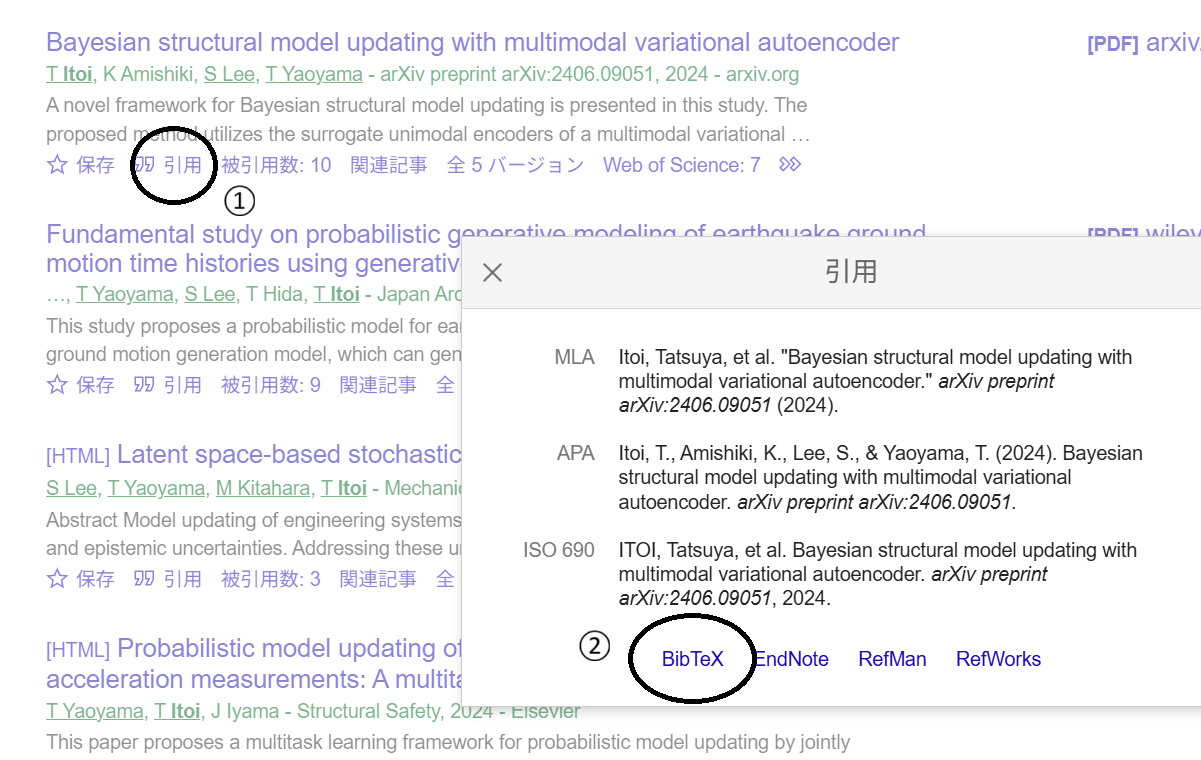
\includegraphics[keepaspectratio, width=100truemm]{figure/scholar.png}
  \caption{Google Scholar の画面}
  \label{fg:scholar}
\end{figure}

.bibファイルの中身を読めばわかるように,\{~\}で囲まれた各文献情報の先頭に,その文献を参照するためのキーを設定しています.
「第一著者名+年」など,わかりやすいキーを設定するようにしましょう.

\subsection{.bibファイルの読み込み}

.bibファイルを反映させるため,呪文を唱えて儀式を行う必要があります.
ただし,VSCode環境ではかなりやりやすくなっているので身構える必要は全くありません.

まず,参考文献を表示したい箇所に以下の4行を書きます.

\begin{verbatim}
  \renewcommand{\bibname}{参考文献}
  \typeout{}
  \bibliography{tutorial.bib}
  \bibliographystyle{junsrt}
\end{verbatim}

それぞれ意味は本.texファイルの該当箇所を参照してください.
次にこれらのコマンドを\TeX に実行してもらうのですが,このときコンパイルを別のメニューで行う必要があります.
Fig. \ref{fg:vscode} に示すように,サイドバーの「\TeX 」-\textgreater「COMMANDS」-\textgreater「Build LaTeX project」と進んで「Recipe: ptex2pdf (uplatex) -\textgreater pbibtex (後略)」
ボタンを押してください.この一連のコンパイル(platex -\textgreater pbibtex -\textgreater platex -\textgreater platex)を行うことでやっとbibtexを読み込み,
参考文献リストや本文中の参照に反映されます.
この作業は.bibファイルを更新するたびに行う必要があります.

\begin{figure}[hbtp]
  \centering
  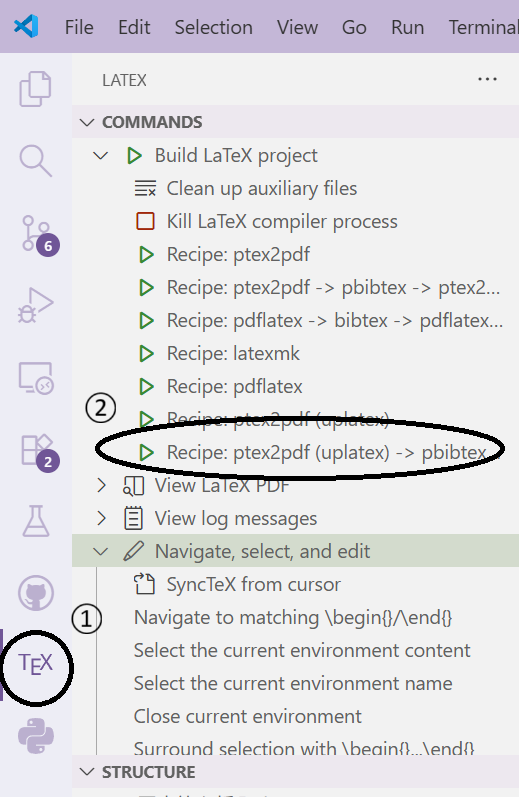
\includegraphics[keepaspectratio, width=60truemm]{figure/vscode.png}
  \caption{VSCode の画面}
  \label{fg:vscode}
\end{figure}

\subsection{参照}

本文中で参照したいときは,\textbackslash cite\{キー\} と書きます.

これは最近公開された論文です\cite{lee2025}.

なお,参照のデザインをプリアンブル内でいじって上付き数字+丸括弧にしてしまいましたが,
いじらない方が論文スタイルとしてよかったかもしれません.

%=====================================================================================

%% 8. 参考文献の作成
\renewcommand{\bibname}{参考文献}
\typeout{} % 謎
\bibliography{tutorial.bib} % bibtexファイルの読み込み
\bibliographystyle{junsrt} % 参考文献表示スタイル

%=====================================================================================

%% 9. 付録の作成
\appendix % 付録の開始

\titleformat{\chapter}{\normalfont\LARGE\bfseries}{付録\thechapter }{1em}{} % 付録のタイトルフォーマット
\renewcommand{\chaptermark}[1]{\markboth{付録\normalfont\thechapter\ ~~#1}{}}

\chapter{付録を書く}
\label{appx:appx}

\renewcommand{\thepage}{\thechapter--\arabic{page}} % ページ数の表記の字体変更(最初の付録だけ)
\setcounter{page}{1} % ページ数リセット

付録を書く際には,ページ数の振り方や章の数え方の法則が本文と異なることに注意が必要です.
付録の章番号は A, B, ..., と進み,ページ番号は A-1, A-2, ..., B-1, B-2, ..., と章ごとにリセットされます.
本.texファイルをテンプレートとして使用すれば問題なく体裁を整えられると思います.

\chapter{別ファイルのソースコードの掲載}
\label{appx:spectrum}

\setcounter{page}{1}

ソースコードを別ファイルで用意して掲載するには,lstinputlisting\{ファイル名\} コマンドを使用します.

\lstinputlisting{response_spectrum.cpp}

%=====================================================================================

\end{document}